% !TeX root = ../main.tex


\chapter{Introduction} \label{chapter:introduction}

Even during the classical era, people have dreamed of inventing machines that can act and think like humans. This opened the field of \textit{artificial intelligence} (AI), which is still an active research topic and is used in many practical applications. The main focus of AI in early days was to solve problems that are hard to solve for humans, such as finding the shortest path to an arbitrary destination using the well-known \textit{Dijkstra algorithm}\footnote{Also known as uniform-cost search}. Ironically, it turned out that tasks, which can be solved by humans using pure intuition, are actually the harder problems to be solved by computers. As an example, it is hard or even impossible to write a program from scratch that is able to detect objects in pictures, recognize words in spoken text or to describe the events in a video scene. The reason is that classical computer programs in contrast have to be algorithmically expressed as a sequence of commands or a list of mathematical rules \parencite{deep_learning}. But it is quite tough to apply this on multi-dimensional data such as pictures or videos that consists of an incoherent set of pixels including different color channels with a lot of noise and countless possibilities. 

Humans handle these kinds of data differently. They learn to recognize objects by experience and implicitly build hierarchies of relationships in their mind. This basic principle opened a new subfield, known as \textit{machine learning} (ML). It covers a methodology where knowledge is acquired by extracting patterns from raw data and consequently allows to make reasonable decisions \parencite{deep_learning}. But while this is able to cover many previously unsolvable problems, it requires that one can tell which features we would like to investigate, for instance to build a decision tree out of it. Coming back to our previous example, this is still hard to be applied on images or video data, where we might know which features we are looking for, but still cannot formally describe how these are represented. A field that deals with these issue is called \textit{representation learning}, which tries to automatically build the representation by itself.

Having just a high-level representation might still not be enough. To divide and conquer this even further, \textit{artificial neural networks} (ANN) have been introduced. They are biologically inspired by the structure of the human brain \parencite{ann} and can be trained to learn hierarchies of representations. For object recognition on images, we can think of edges that are detected on a very low level, which will be further composed to curves or shapes. Moreover, these simple structures might be compound in a specific way, so that the neural network can identify distinct complex objects in it. The rise of computational power allows to create networks that are even deeper and therefore learn more and more complex representations hierarchies. This principle caused its contemporary name, known as \textit{deep learning}.

\section{Motivation}

In recent years, the field of deep learning achieved considerable success and according to its underlying philosophy, ``\textit{if we have a reasonable end-to-end model and sufficient data for training it, we are close to solving the problem.}'' \parencite{conv_lstm_nowcasting}. But while there has been done a lot of studies and practical application of object recognition on static images or speech recognition, the application of these concepts on video data is just about to make its first steps in research. 

First deep learning approaches dealing with video data or simple image sequences address problems like human action recognition \parencite{conv3d_action_class}, \parencite{two_stream_action}, \parencite{longterm_rec_recog} or video classification \parencite{large_video_class}, Another example is optical flow prediction \parencite{flownet} in order to detect the visual flow from one frame to the next. Most of these approaches require lots of labeled data to be able to train a network. The effortful labeling process and thus the resulting low availability of such data might be the main reason why this topic has not been covered that well so far. On the contrary, online services like \textit{YouTube} provide a seemingly endless, but unlabeled source of videos to learn from.


\section{Problem Statement}

Throughout this work, we would like to investigate whether deep learning techniques can be successfully applied on videos to learn a meaningful representation in a completely unsupervised fashion. In detail, we would like to examine if such a representation is suited to continue a video even after is has finished. Hence, to learn a notion of the spatial and temporal evolution within a sequence of images as well as to get an idea of motion and dynamics of a scene. Such a high-level understanding would be helpful for autonomous intelligent agents that have to act and therefore understand our environment including its physical and temporal constrains \parencite{unsup_learn_lstm}. Other application areas might be for instance video compression \parencite{frame_interpol}, visual systems for autonomous cars or as a replacement for optical flow in causal video segmentation \parencite{causal_video_seg}. Aside from that, other supervised learning tasks like human action recognition could benefit from such a pre-trained network in order to improve the overall performance or to reduce the training time. Needless to say, other forms of \textit{transfer learning} are easily conceivable as well.

\begin{figure}[htpb]
	\centering
	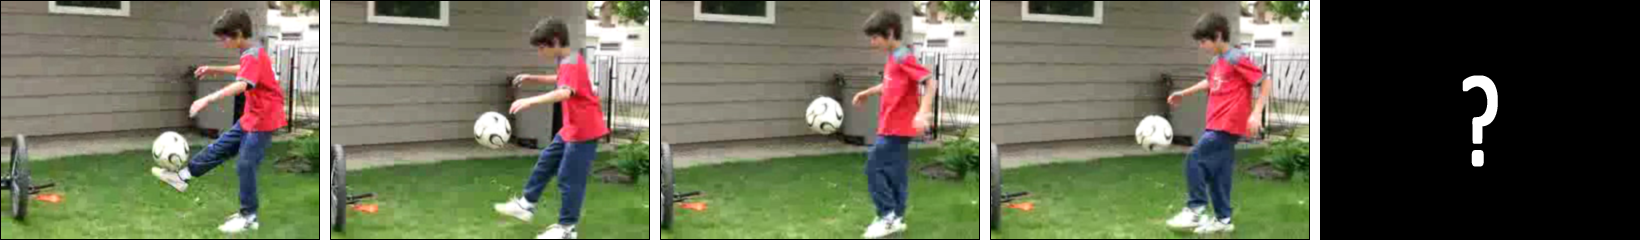
\includegraphics[width=1.0\linewidth]{figures/ucf-intro/serie1.png} 
	\caption[Example Image Sequence]{Example of an image sequence (starting from the left) with an unknown future frame.} \label{fig:intro-seq}
\end{figure}

Like in the first example of object recognition on static pictures, this task might sound trivial for humans once more, since we already have built an intuition regarding motion and our environment. When we have a look at the image sequence in Figure \ref{fig:intro-seq}, we have a strong idea about how this sequence might continue. At least for a couple of time steps. The boy in the foreground probably will lift his left foot towards the ball, while the ball continues to fall down due to gravitation. In contrast, the background will stay almost unchanged.

Developing a deep learning approach to tackle this is indeed a non-trivial task, as it has to model both, spatial and temporal features in combination. Additionally, related issues like evolving an effective training process or quantifying the perceptual image similarity between predicted and the ground truth frames have to be addressed as well. Moreover, existing state-of-the-art implementations that deal with frame prediction have to be reviewed and analyzed in detail in order to learn from their strength and weaknesses.


\section{Contributions}

This thesis consists of several contributions. Firstly, it provides a dense \textit{overview} of existing deep learning approaches that deal with the problem of future frame prediction in videos. Secondly, we present a neural network architecture that combines modern practices like \textit{batch normalization} with a novel \textit{convolutional LSTM} implementation and \textit{scheduled sampling} to improve training of recurrent models. Thereby, we are able to \textit{cut in half the prediction error} of other state-of-the-art models in the MovingMNIST dataset. Last but not least, we make all of our TensorFlow implementations available to the research community, including our scheduled sampling and batch normalization enabled convolutional recurrent cell, as well as several metrics and loss functions to measure perceptual image similarity at training time. Further, we contribute an \textit{lightweight, high-level and open source framework for TensorFlow} that is able to radically reduce boilerplate code of deep learning applications. This is facilitated by providing an abstraction for many recurring or complex tasks that have to be faced while building and training neural network models.


\section{Organization}

The subsequent chapters of this thesis are structured as follows:

\textbf{Chapter \ref{chapter:fundamentals}} covers the theoretical concepts that are required to understand our final implementation and its consecutive evaluation. We will have a deeper look into neural networks and explain how they are trained. Further, we will explore more advanced neural network architectures, namely \textit{convolutional neural networks} (CNN) for spatial learning and \textit{recurrent neural network} (RNN) models for sequential learning. Afterwards, we conclude this chapter with the investigation of some modern techniques that are used to improve the overall learning process, as well as metrics for perceptual motivated image similarity assessment.

In \textbf{Chapter \ref{chapter:relatedwork}}, we take a closer look at existing approaches that are suitable for spatio-temporal learning and frame prediction. We briefly discuss their strength and weaknesses, as well as how they have influenced the design decisions regarding the architecture of our final neural network model. Additionally, these presented models build the baselines in our evaluation.

Afterwards, we present our neural network model in \textbf{Chapter \ref{chapter:implementation}}, including its architecture and implementation details. Moreover, we introduce a quite recently introduced and barely studied variant of recurrent network cell for spatio-temporal learning, namely \textit{convolutional LSTM}, which builds the central element of our model. We also suggest a special learning strategy for RNNs, which speeds up the training process and enables to improve the overall performance.

\textbf{Chapter \ref{chapter:datasets}} gives a brief overview of the video datasets used within this thesis. All in all, we have chosen three different sets with increasing complexity, namely \textit{Moving MNIST}, \textit{MsPacman} and \textit{UCF-101}.

Next, \textbf{Chapter \ref{chapter:evaluation}} illustrates many experimental results on the previously named datasets. We investigate how changes in the model or hyperparameters do affect the model's performance, as well as compare our results with other existing approaches in detail.

With \textbf{Chapter \ref{chapter:contribution}}, we would like to present a lightweight, high-level framework for \textit{TensorFlow} as a side contribution that has grown out of this project.

In the end, we conclude this thesis in \textbf{Chapter \ref{chapter:conclusion}} by summarizing our results and outcomes, as well as highlight the identified possible improvements for future work.



